{\color{red} DOCSIS}\\

Es una tecnología desarrollada por CableLabs para la transferencia de datos a través de cable coaxial que se implementan y utilizan para la conexión de televisión por cable. Los operadores de cable de todo el mundo han adoptado los estándares DOCSIS para proporcionar servicios de datos, voz y video de Internet utilizando los sistemas de televisión por cable existentes.\\

DOCSIS funciona principalmente entre las capas 1 y 2 del modelo OSI (Capa Física y Capa de Control de Acceso al Medio). En términos simples, las redes DOCSIS son redes IP sobre HFC, donde los paquetes IP son codificados y transportados como señales de televisión digital que coexisten con otros servicios también transportados por la red. 

\section*{Downstream: Desde el CMTS hacia los CM}
La banda de downstream se comparte con los demás servicios que brinda la red. El ancho de banda para cada canal descendente puede ser de 6 MHz o de 8 MHz para cumplir con las normas de los canales de difusión de televisión en Norteamérica y Europa. Los formatos de modulación que pueden ser empleados son: 64-QAM y 256-QAM. \\

Los paquetes enviados por el canal de bajada se separan en tramas MPEG (Moving Picture Experts Group) de 188 bytes, con 4 bytes de encabezado y 184 bytes de carga útil. Aun cuando a todos los CM llegan todas las tramas, normalmente se configuran para recibir solamente las que están direccionadas a su dirección MAC o a la dirección de difusión. \\

En el sentido descendente, DOCSIS emplea un sistema primero-que-llega primero-que-seatiende para el reenvío de paquetes, así los paquetes que arriban de Internet se reenvían inmediatamente como paquetes DOCSIS.

\section*{Upstream: Desde los CM hacia el CMTS}

Las características de esta banda (ruido y distorsión) hacen que se necesiten mecanismos robustos, como modulaciones eficientes, para la transmisión de datos. A diferencia de la banda de downstream, en la que sólo hay un transmisor, en esta banda hay muchos transmisores y un solo receptor, por lo que la utilización del medio de transmisión deber ser cuidadosamente organizada y repartida entre todos los CM. Por todo esto se conforman los CMTS con más puertos de subida que de bajada, permitiendo segmentar más la red en el sentido ascendente y lograr mejores niveles de señal.\\

Los tipos de modulación establecidos para los moduladores/demoduladores de upstream son: QPSK (Quadrature Phase-Shift Keying), 8-QAM (Quadrature Amplitude Modulation), 16QAM, 32-QAM, 64-QAM y 128-QAM. El CMTS reserva el ancho de banda de upstream basado en peticiones de los CM y las políticas de calidad de servicio. El canal de subida se divide en ranuras de tiempo multiplexadas, llamadas mini-slots, de una duración de 6.25 $\mu$s, y la oportunidad para transmitir en ellas es administrada por el CMTS, que las identifica mediante referencias de tiempo y que son utilizadas por los CM según mecanismos de contención. La influencia de la distancia en el retardo implica una compensación de tiempo (offset) en las referencias de los CM para que identifiquen con suficiente precisión la posición de los mini-slots.\\

Básicamente, para que funcione la red DOCSIS se debe tener en funcionamiento el CMTS, un servidor DHCP y uno TFTP, para que los CM puedan registrarse.\\

Cuando un CM se conecta a la red coaxial, y se enciende, comienza a rastrear un canal descendente buscando en toda la banda una transmisión 64-QAM o 256-QAM, que contenga información válida acerca de un canal de subida, para poder establecer una comunicación bidireccional. Si efectivamente lo encuentra y lo retiene, comienza lo que se conoce como Ranging. El Ranging es un proceso que consta de dos etapas, la primera es el Ranging Inicial, en la que se configura el menor nivel de potencia que garantiza la comunicación. Después pasa a un nuevo estado conocido como Ranging de Mantenimiento (Station Maintenance Ranging), en el que el CM recibirá instrucciones desde el CMTS para hacer ajustes. El Ranging de Mantenimiento de Estaciones ocurrirá al menos una vez cada 30 segundos para cada CM, realizando ajustes de forma continua y para que el CMTS conozca que los módems se encuentran en línea.\\

De esta manera, el CMTS periódicamente envía tramas de gestión y otra clase de mensajes denominados mensajes MAP, para que los CM puedan identificar futuras ranuras TDMA para el canal upstream. Inmediatamente al contar con ancho de banda para transmitir, el CM obtiene su IP y otras direcciones importantes mediante DHCP y descarga el archivo de configuración del servidor TFTP, con los parámetros que necesita para el acceso a la red, velocidades, QoS y otras configuraciones. Si las pruebas de validez son satisfactorias, se concluye el proceso con el Registro del CM en la red y se le asigna un identificador de Servicio (SID). Una vez registrado el CM, se permite a los suscriptores transmitir tráfico IP

\begin{figure}[ht!]
\centering
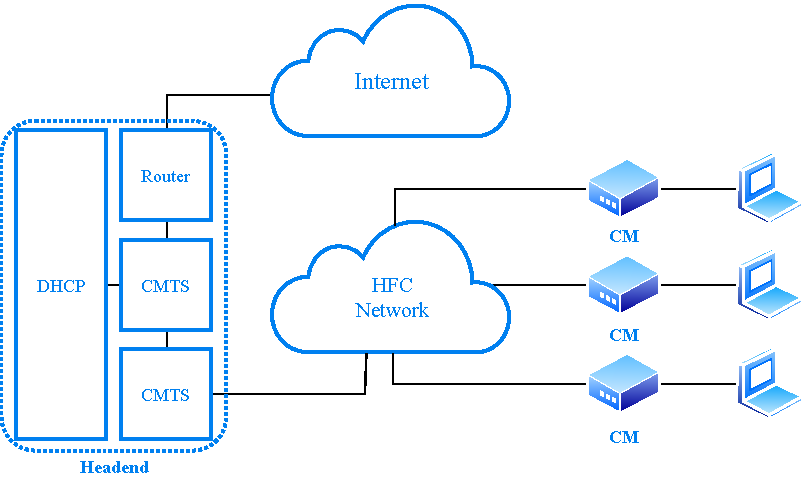
\includegraphics[scale=0.66]{Imagenes/docsis.pdf}
\end{figure}



\section*{Frecuencias a las que funciona DOCSIS}
DOCSIS garantiza su adecuado funcionamiento en las redes de cable que adoptan el estándar. Además de ser un estándar de interoperabilidad de cable módem, DOCSIS incluye parámetros que se recomiendan para lograr un mejor desempeño de la red de cable. Los rangos de frecuencia que utiliza DOCSIS en las redes bidireccionales son:

\begin{figure}[ht!]
\centering
\includegraphics[scale=0.66]{Imagenes/tablaDOCSIS.png}
\end{figure}

\section*{Inicialización del Sistema}
Dentro de los aspectos a considerar en la inicialización que realiza el CM se encuentran las siguientes tareas que debe realizar previo al paso de información a través de la red:

\begin{itemize}
\item Examina el canal descendente y establece la sincronización con CMTS. 
\item Obtiene los parámetros para la transmisión. 
\item Analiza el rendimiento del proceso Ranging. 
\item Establece la conectividad IP a través de DHCP. 
\item Establece parámetros de tiempo. 
\item Transfiere los parámetros operacionales de transmisión vía el protocolo TFTP. 
\item Registra al CMTS
\end{itemize}

\section*{Proceso de Entrega al CM}
Dentro de las funciones que realiza el CM para la entrega y recepción de información se tienen los siguientes:
\begin{itemize}
\item Encapsula el flujo de bits en paquetes Ethernet provenientes del canal downstream.
\item La señal recibida por el canal descendente es demodulada para extraer los datos del usuario y la información de señalización y control que envía el equipo cabecero.
\item Convierte los paquetes Ethernet en tramas según lo definan las capas MAC.
\item Los datos originados por el usuario son extraídos de los paquetes Ethernet que llegan al ordenador y se encapsulan formando otro tipo de paquetes cuyo formato dependerá del protocolo de red empleado; en el sistema de CM, los paquetes son transmitidos en el instante y el canal indicado por la cabecera.
\item La cabecera ha de disponer de unos equipos que realicen funciones de router y switch, y que adapten el tráfico de datos de la red HFC al protocolo IP. Además, debe existir un sistema de gestión de red y de abonados.
\end{itemize}

\section*{Versiones de DOCSIS}

Durante las últimas dos décadas, la tecnología DOCSIS ha evolucionado desde la versión 1.0 inicial con velocidades máximas de 42 Mbps a DOCSIS 3.0, que puede proporcionar velocidades de 100 Mbps para servicios de Internet, telefonía y video.


\subsection*{DOCSIS 1.0}
DOCSIS 1.0 fue diseñado para uniformar el alto rendimiento de suministro de acceso a Internet permitiendo que los operadores de cable puedan capitalizar oportunidades de prestación de servicios diferentes a más de estandarizar la comunicación entre el CMTS y el CM, reducir la complejidad y abaratar costos. Inicialmente los beneficios que presentó DOCSIS 1.0 fueron reducidos, pero en forma general atractivos para los operadores que buscaban el mejoramiento de la calidad de servicio en la red de cable, seguridad, escalabilidad e interoperabilidad de la misma.

\subsubsection*{Características}
\begin{itemize}
\item Emplea modulación 64-QAM en el canal descendente.
\item Utiliza modulación QPSK en el canal ascendente.
\item Utiliza como archivo de configuración del cable módem a TFTP (Protocolo de Transferencia de Archivos de Texto).
\item Maneja el protocolo de configuración de huésped dinámico (DHCP), para la asignación de direcciones IP dinámicamente.
\item Para la corrección de errores se vale de FEC (Corrección Progresiva de Errores).
\item Puede ser programado para trabajar con el algoritmo Reed-Solomon.
\end{itemize}
\subsubsection*{Servicios}
\begin{itemize}
\item Conectividad a Internet básico. 
\item Servicio gradual de datos con calidad de servicio por módem. 
\item Red virtual privada (VNPs) a los proveedores de servicio upstream (ISPs) 
\end{itemize}
\subsection*{DOCSIS 1.1}
DOCSIS 1.1 fue introducido para proveer a la industria una especificación de suministro mejorado de datos a través de la red de cable. Esta estandarización facilita muchos beneficios a los operadores, vendedores y consumidores. La interoperabilidad es un beneficio clave ya que permite al operador construir y avanzar más fácilmente sobre infraestructuras que permitan ofrecer servicios perfeccionados que tienden a fortalecer la competitividad. DOCSIS 1.1 fue introducido al mercado para satisfacer los requerimientos más exigentes de los usuarios, mejorar la calidad de servicio, y poder introducir nuevas aplicaciones sobre la red existente.
\subsection*{Característica}
DOCSIS 1.1 es un conjunto de especificaciones que incorpora características de Calidad de Servicio (QoS) y autenticación, necesaria para manejar servicios que requieren una entrega de datos en tiempo real y mayor seguridad como es el caso de la telefonía.
\begin{itemize}
\item La velocidad de transferencia de información es de 10.24 Mbps en el canal ascendente.
\item Realiza fragmentación de datos evitando de esta forma que un CM grande monopolice el canal ascendente durante un intervalo de tiempo.
\item Emplea modulación 16-QAM en el canal ascendente. 
\item Utiliza modulación 256-QAM en la canal descendente.
\item Parámetros de calidad de servicio QoS introducidos con la clasificación del tráfico para dar mayor flexibilidad.
\item DOCSIS 1.1 provee para la corrección de hasta 10 bytes errados a través del algoritmo de Reed-Solomon (RS) (T=10).
\end{itemize}
\subsubsection*{Servicios}
\begin{itemize}
\item Servicios en tiempo real (VoIP).
\item Multimedia, video, juegos online, donde se compromete los parámetros de calidad.
\item Servicio a proveedores de Internet (ISPs), detrás del mismo cable módem.
\item Televisión Interactiva. 
\item Video bajo demanda. 
\item Videoconferencia. 
\item Datos.
\end{itemize}

\subsection*{DOCSIS 2.0}
DOCSIS 2.0 fue desplegado para mejorar la eficiencia de banda ancha y el rendimiento en las redes de cable, su desarrollo se da específicamente en atención a la industria de cable afectada por la limitación de capacidad del canal upstream y la vulnerabilidad a deterioros de ruido.
\subsubsection*{Características}

\begin{itemize}
\item Velocidad de transferencia de información es de 30.72 Mbps en el canal ascendente. 
\item Maneja QoS. 
\item Mayor inmunidad al ruido. 
\item Máximo ancho de banda del canal 6.4 MHz. 
\item Utiliza modulación 256-QAM en el canal ascendente. 
\item Emplea modulación 256-QAM en el canal descendente.
\item Se puede ofrecer servicios simétricos.
\item Mayor protección contra daños electrónicos. 
\item Compatibilidad total con cable módems (CM) DOCSIS 1.0 y 1.1 y Sistema de Terminación de Cable módem (CMTS).
\item DOCSIS 2.0 facilita la fragmentación de paquetes de datos.
\end{itemize}

\subsubsection*{Servicios}

\begin{itemize}
\item Voz sobre IP. 
\item Trabajo en red par-a-par. 
\item Videoconferencia. 
\item Video bajo Demanda. 
\item Televisión Interactiva. 
\item Multimedia. 
\item Datos
\end{itemize}

\subsection*{DOCSIS 3.0}
DOCSIS 3.0 consiste en una serie de especificaciones que define la tercera generación de la transmisión de datos de alta velocidad sobre sistemas de cable. Fue expedida en la primera semana de agosto de 2006 y representa la gran evolución del estándar. La flexibilidad en la implementación de sus nuevas características y la escalabilidad de los equipos de terminación lo hacen muy atractivo. La principal característica que aporta la versión 3.0 de DOCSIS es el Channel Bonding, que permite agrupar varios canales físicos para formar un gran canal lógico y aumentar el ancho de banda, tanto en subida como en bajada para cada suscriptor.


\begin{figure}[ht!]
\centering
\includegraphics[scale=0.66]{Imagenes/tabla_comparacion.png}
\end{figure}

\begin{thebibliography}{9}
\bibitem{tutorialspoint} 
Descripción del estándar DOCSIS y sus aplicaciones en las redes HFC. Universidad Central “Marta Abreu” de Las Villas. 2016.

\bibitem{docsis}
Meet DOCSIS, Part 1: the unsung hero of high-speed cable Internet access. \href{https://arstechnica.com/information-technology/2011/05/docsis-the-unsung-hero-of-high-speed-cable-internet-access/}{https://arstechnica.com/information-technology/2011/05/docsis-the-unsung-hero-of-high-speed-cable-internet-access/}

\bibitem{doc}
DOCSIS 3.1 Technology Whitepaper, NETGEAR.

\end{thebibliography}

